\section{Analyse existierender Ansätze zur Dokumentähnlichkeitsbestimmung basierend auf Bayesscher Statistik}
\label{sec:AnalyseAnsätze}


\subsection{More Like This}
\label{subsec:MLT}

Der More Like This (MLT) Algorithmus ist, ein Algorithmus, der es ermöglicht Dokumente zu finden, die ähnlich sind zu den Dokumenten einer Ergebnisliste. Das Ganze läuft durch Relevanz-Scoring, wo Dokumente auf Relevanz geprüft werden. Um eine optimale Gestaltung des Relevanz-Scoring zu erzielen, das Algorithmus verringert die Anzahl an Kandidaten Dokumente durch einen Boolean Test, bei dem das gesuchte Dokument vergleicht wird mit der Abfrage. Die durch Boolean Test selektierte Dokumente werden Punkte erhalten. Die Bestimmung des Rangs für die Relevanz wird auf Basis diesen Punkten erfolgen. Ein Dokument kann trotz eine Übereinstimmung irrelevant sein für die Abfrage. Deswegen ist die Einstellung einer Filterung von Übereinstimmungen nach Index, dokumenttyp oder durch kontextueller Logik wichtig zur Lösung dieses Problems.
Die Bewertungsfunktion der Informationsabrufsoftware-Bibliothek Lucene wird bei dem MLT Algorithmus genutzt. Diese entspricht ein auf der Begriffsfrequenz und der Inverse Dokumenthäufigkeit basierende Ähnlichkeitsmodell, das das Vektorraummodell für mehrere Begriffe Abfragen benutzt. Es sind unterschiedliche Ähnlichkeitsalgorithmen verfügbar:
\begin{itemize}
	\item [(1)]BM25 okapi: diese basiert auf die Begriffsfrequenz/inverse Dokumenthäufigkeit. Die Steuerung sowohl von nichtlineare Begriffshäufigkeitsnormierung als auch des Normalisierungsgrades von Begriffsfrequenz-Werte durch die Dokumentlänge. 
\item[(2)] die klassische Ähnlichkeit: basiert auch auf Begriffsfrequenz/inverse Dokumenthäufigkeit. Sie bestimmt, ob Überlagerungstoken bei der Berechnung der Norm ignoriert werden\cite{ELA18}.
\begin{itemize}
	\item [(3)]	die Abweichung von Zufälligkeitsähnlichkeit
\item [(4)]	Abweichung von der Ähnlichkeit der Unabhängigkeit, 
\item [(5)]Informationsbasierte Ähnlichkeit
\item [(6)]	Skriptähnlich Ähnlichkeit: die Verwendung eines Skriptes zur Angabe wie die Ergebnisse berechnet werden sollen \cite{ELA18}.
\item [(7)]	LM Jelinek Mercer Ähnlichkeit: die Erfassung von wichtigen Muster im Text mit Rücksichtlosigkeit von Rauschen.
\item [(8)]	LM Dirichlet Ähnlichkeit
\end{itemize}
\end{itemize}
\subsection{Naive Bayes}
\label{subsec:NB}


\subsection{BayesLSH}
\label{subsec:BayesLSH}

%The interaction between enterprises' applications has suffered in the past from lack of standardized technologies, leading each of the enterprises to develop their own or acquiring vendor-specific integration technology. \ac{JBI} is defined by the Java Community as an integration technology which maximizes the decoupling between components and defines an interoperation semantic founded on standards-based messaging. This allows different vendor-specific components to interoperate in a multivendor "echosystem" \cite{JBI2005}. 

%The key which leads to the integration of different components relies on a unique message format in the \ac{JBI} environment which different plugged-in components use to communicate within the environment. External components are not directly connected, but through a mediator. The communication mediator between components in a \ac{JBI} environment is the \ac{NMR}. Its main functionality is the routing of the internal standardized \ac{NM} between the components. However, it can perform additional processing during the message exchange. The \ac{NMR} fields are defined as an \ac{XML} document format payload, metadata conforming the header and a non \ac{XML} document format attachment referenced by the payload.

%The \ac{JBI} specification defines two different types of components which are categorized in two types and provide different services:
%	\begin{itemize}
%		\item A \ac{SE} provides transformation and composition services to other components.
%		\item A \ac{BC} provides the connectivity between the external services and the \ac{JBI} environment. They support many different protocols and isolate the \ac{JBI} environment by marshaling and demarshaling the incoming or outgoing message into the internal standardized \ac{NM} format.
%	\end{itemize} 
	
%Both components listed above can function as service consumers or service providers following a \ac{WSDL}-based, service-oriented model. The consumer endpoint provides a service accessible through an endpoint which can be consumed by other components, while the provider endpoint consumes a functionality exposed as a service and accessible through an external endpoint. The routing of \ac{NM} starts when a message exchange between components is created (bidirectional communication pipe, a \term{DeliveryChannel}, between the communicating endpoints) and continues with the target of the specified service endpoint for processing (see Figure \ref{fig:jbi}). The \ac{NMR} supports four asynchronous message exchange patterns differing in the reliability and direction of the communication.

%\begin{figure}[htb]
%	\centering
%		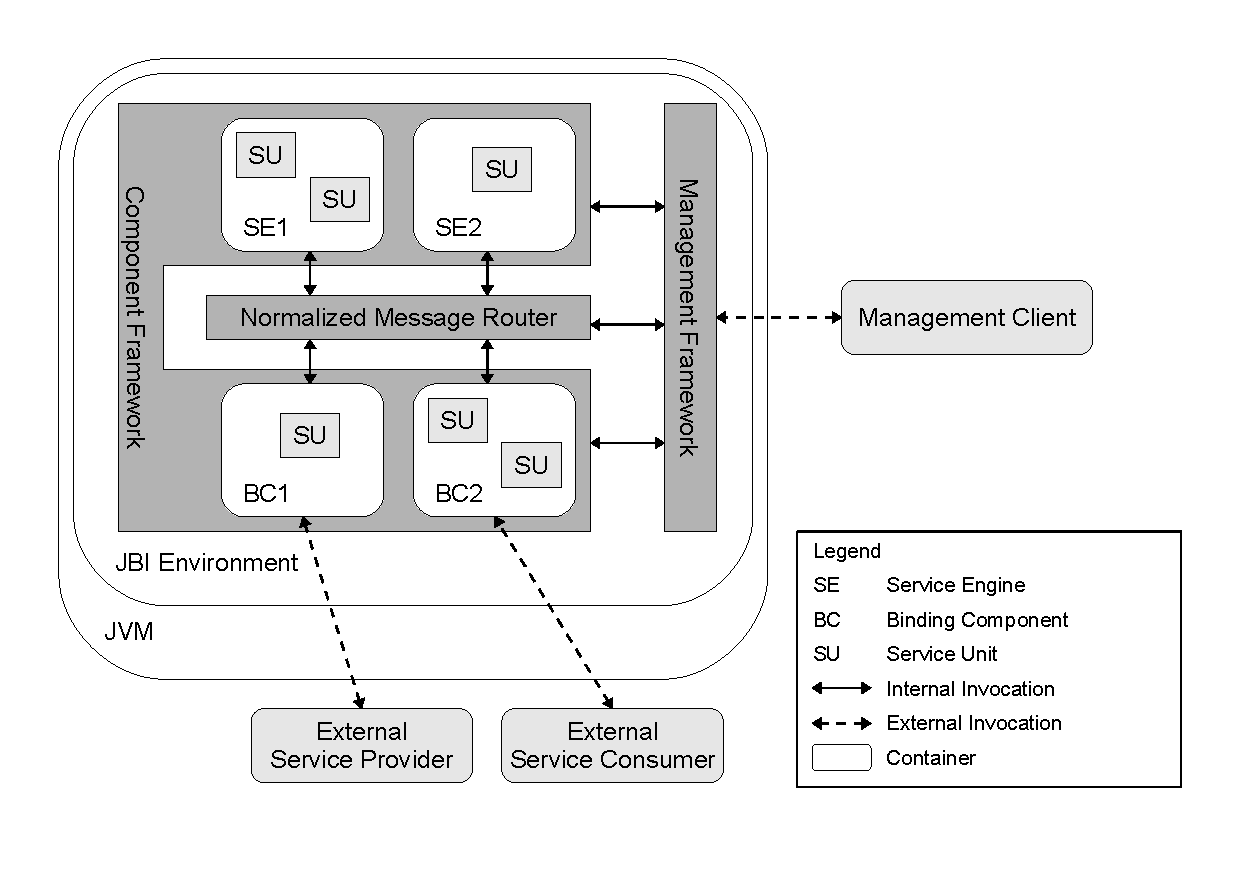
\includegraphics[width=0.85\textwidth, trim=0.95cm 0.95cm 0.95cm 0.95cm, clip]{./gfx/JBIArchitecture.pdf}
%	\caption[JBI Architecture]{Overview of JBI Architecture. Figure 4 in JBI specification document \cite{JBI2005}.}
%	\label{fig:jbi}
%\end{figure}

%In Figure \ref{fig:jbi} we can observe that one or more \ac{SU} are contained in a \ac{BC}. The \ac{SU}s are component-specific artifacts to be installed to a \ac{SE} or a \ac{BC} \cite{JBI2005}. The service units are packed in a \ac{SA}, usually as ZIP files, where it is specified each of the components where each of the \ac{SU}s should be deployed. The \ac{JBI} environment provides a Java Management Extension \ac{JMX} Framework for installation, life cycle management, addition, and monitoring and control of the components conforming to the environment defined by the JBI specification.

%\FloatBarrier